实验表明，对于连续砂床或严重出砂井况，常规水力冲砂冲砂效率低，除砂效果差。针对此难题，本章主要开展水力脉冲冲砂洗井工具结构设计并阐述冲砂洗井工具的结构组成和工作原理，然后建立水力脉冲脉冲洗井工具数学模型并通过CFD仿真验证工具的冲砂效果。

\subsection{水力脉冲冲砂洗井工具结构组成}

水力脉冲冲砂洗井工具主要由脉冲发生模块与旋转喷头模块构成,如图\ref{fig:tool_structure_3_in_1}所示。旋转喷头模块的核心功能在于利用前向布置的高压喷嘴产生强力射流，直接作用于井底沉积砂床，通过流体的高剪切应力实现对砂床表面的破坏与砂砾的卷扬，使沉积颗粒在卷扬作用下重新进入悬浮运移状态；同时，配合周向旋转机构实现的 全覆盖喷射，消除了常规清洗中的水力死角。脉冲模块则负责产生一种具有低频特性的高、负压交替水力冲击波。该模块通过对油套管内壁进行高频次的反复激励，利用压力脉动产生的振动效应有效疏通并剥离附着于管壁的坚硬垢层与残留杂质。更为关键的是，水力冲击波在环空流体中传播时，能为已沉积或趋于沉积的砂砾提供额外的扰动动能，破坏颗粒间的动力平衡状态，从而显著提升井筒清砂的整体作业效率。

\begin{figure}[htbp]
	\centering
	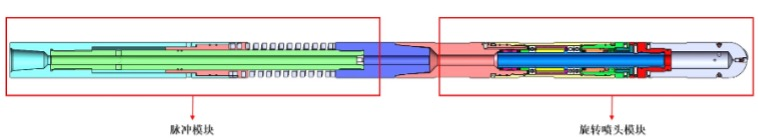
\includegraphics[width=1.\textwidth]{figure/chapter3/tool-structure-3-in-1.jpg}
	\caption{水力脉冲冲砂洗井工具结构示意图}
	\label{fig:tool_structure_3_in_1}
\end{figure}

\subsection{水力脉冲冲砂洗井工具结构设计及工作原理}

\subsubsection{水力脉冲冲砂洗井工具旋转喷头模块设计}
如图\ref{fig:nozzle_sub}所示，旋转喷头模块主要由上接头、筒体、芯轴、连通隔套、平衡活塞、底部帽、平衡活塞座、喷头连接体、隔套、座、旋转喷头、喷嘴和骨架油封等密封件以及轴承和复位弹簧等零部件组成。其工作原理是旋转喷头模块位于工具作业串的最前端，用钻杆送入至指定的位置，其余工具固定好之后，开泵循环泵入介质，流体由工具上接头导入，沿中心芯轴流道行进，最终经由端部喷嘴高速喷出。在此输运过程中，由于工具内部流道截面积缩小，流体节流从而产生巨大压降，流速增快从而产生冲击效果。此外，为实现全向清洗，喷头结构中设计了两组具有特定偏心夹角的喷嘴。当高速介质经由倾斜流道射出时，射流产生的反冲推力在工具横截面上形成持续的偏心力矩，该力矩直接驱动旋转喷头与芯轴自转，进而实现对套管内壁 360° 无死角的周向清洗。

\begin{figure}[htbp]
	\centering
	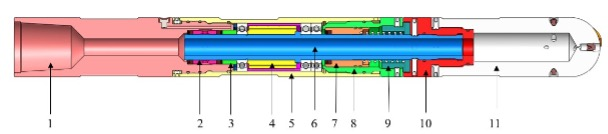
\includegraphics[width=1.0\textwidth]{figure/chapter3/nozzle-sub.jpg}
	\caption{水力脉冲冲砂洗井工具结构示意图}
	\label{fig:nozzle_sub}
\end{figure}

\subsubsection{水力脉冲冲砂洗井工具脉冲发生模块设计}

如图\ref{fig:pulse_module}所示，脉冲发生模块由上接头、芯轴、移动活塞、矩形弹簧、下接头组成。其工作原理是脉冲发生模块圆周上设计有出水孔，靠地面泵或注水管线，把液体传入井下，水流通过节流喷嘴时会产生节流压差，对脉冲器活塞面产生高压作用。

\begin{figure}[htbp]
	\centering
	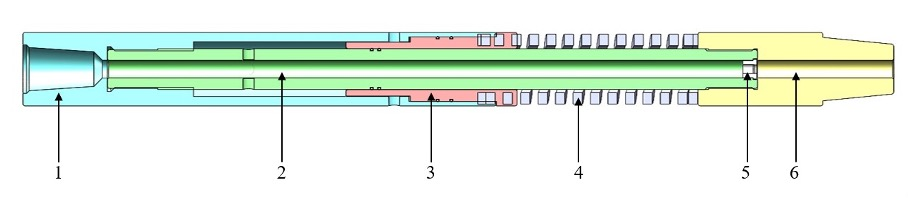
\includegraphics[width=1.0\textwidth]{figure/chapter3/pulse-module.jpg}
	\caption{水力脉冲冲砂洗井工具脉冲发生模块结构图}
	\label{fig:pulse_module}
\end{figure}


脉冲发生模块的工作原理如\ref{fig:principle_of_pulsing_tool}所示。在高压作用下，活塞克服矩形弹簧的预紧力及流体的粘滞及摩擦阻力产生轴向位移，当活塞上端面到达侧向出水孔时，侧向出水孔开启，高压水射流从侧向出水孔喷出，腔内压力开始下降，活塞在弹簧压缩力的作用下开始复位，侧向出水孔关闭。活塞复位到初始位置，系统开始下一循环。

该装置向井筒环空传递振动能量的途径主要包括两种机制：首先是振动器本体产生的轴向机械振荡；其次是由高压脉冲流体激发的径向水力冲击效应。在上述复合动载荷的共同叠加下，环空内的局部流场呈现出强烈的瞬态扰动特性。原本压实沉积的砂床结构被脉冲射流破坏，砂粒由静态沉降转变为悬浮流化状态，进而配合循环工作液被高效排出井筒。

\begin{figure}[htbp]
	\centering
	\subfloat[脉冲发生模块蓄能阶段]{%
	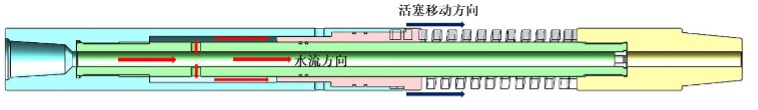
\includegraphics[width=0.9\textwidth]{figure/chapter3/energy-storage-in-pulse-module.jpg}
	}
	\vspace{1em}
	\subfloat[脉冲发生模块复位阶段]{%
	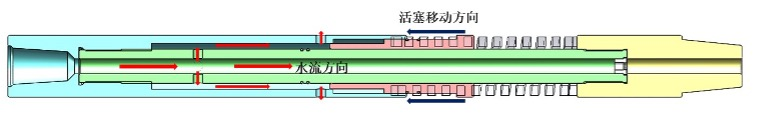
\includegraphics[width=0.9\textwidth]{figure/chapter3/restore-in-pulse-module.jpg}
	}
	\caption{脉冲发生器工作原理}
	\label{fig:principle_of_pulsing_tool}
\end{figure}

\subsubsection{毛刷刮管模块设计}

MSQ型毛刷刮管器是用于清除井下套管内壁上的残余水泥，泥块、生产井套管上的铁锈，水垢，硬石蜡等影响正常施工作业杂物的工具。MSQ型毛刷刮管器主要由上接头、上扶正套、毛刷体、下扶正套、剪切套、剪切定位套、下接头等部件组成。其工作时主要靠上毛刷和下毛刷对刮削过的套管内壁进行刷洗清洁。在浅井内工作时主要靠下毛刷对套管内壁进行刷洗清洁，当刮削到一定深度后，下毛刷发生磨损后上毛刷体可自动伸出参与刷洗清洁，从而保证在整个作业过程中套管清洁的质量。

\begin{figure}[htbp]
	\centering
	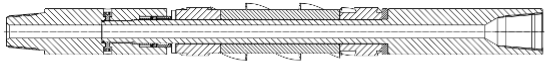
\includegraphics[width=0.9\textwidth]{figure/chapter3/swiper-in-3-in-1.png}
	\caption{毛刷刮管器结构简图}
	\label{fig:swiper_in_3_in_1}
\end{figure}

工具的技术参数如下表所示。


\begin{table}[htbp]
    \centering
    \caption{脉冲器技术参数}
    \label{tab:pulsar_params}
    \renewcommand{\arraystretch}{1.5} % 增加行高，使表格更美观
    \begin{tabularx}{1.\textwidth}{cXcccccc}
        \toprule % 顶线
        代号 & 适用套管规格 & \begin{tabular}[c]{@{}c@{}}组装外径\\ (mm)\end{tabular} & \begin{tabular}[c]{@{}c@{}}最小通径\\ (mm)\end{tabular} & \begin{tabular}[c]{@{}c@{}}长度\\ (mm)\end{tabular} & \begin{tabular}[c]{@{}c@{}}最大抗拉\\ (kN)\end{tabular} & \begin{tabular}[c]{@{}c@{}}最大抗扭\\ ($\text{kN}\cdot\text{m}$)\end{tabular} & 连接螺纹 \\
        \midrule % 栏目线
        MSQ105 & $4-1/2''$ & 105 & 25 & 1250 & 912 & 14.2 & \begin{tabular}[c]{@{}c@{}}NC31\\ ($\text{P}\times\text{B}$)\end{tabular} \\
        \bottomrule % 底线
    \end{tabularx}
\end{table}

\begin{table}[htbp]
    \centering
    \caption{旋转喷头技术参数}
    \label{tab:rotary_nozzle_params}
    \renewcommand{\arraystretch}{1.5} % 增加行高，使表格更美观
    \begin{tabularx}{1.\textwidth}{ccccccccc}
        \toprule % 顶线
        \begin{tabular}[c]{@{}c@{}}外径\\ (mm)\end{tabular} & 
        \begin{tabular}[c]{@{}c@{}}总长\\ (mm)\end{tabular} & 
        \begin{tabular}[c]{@{}c@{}}喷嘴尺寸\\ （mm $\times$ n）\end{tabular} & 
        \begin{tabular}[c]{@{}c@{}}工作排量\\ (L/min)\end{tabular} & 
        \begin{tabular}[c]{@{}c@{}}转速\\ (r/min)\end{tabular} & 
        \begin{tabular}[c]{@{}c@{}}工作压强\\ (MPa)\end{tabular} & 
        扣型 & 
        \begin{tabular}[c]{@{}c@{}}最大抗拉\\ (kN)\end{tabular} & 
        \begin{tabular}[c]{@{}c@{}}最大抗扭\\ ($\text{kN}\cdot\text{m}$)\end{tabular} \\
        \midrule % 栏目线
        105 & 1045 & $3.175 \times 7$ & 100-500 & 10-300 & $\le 70$ & \begin{tabular}[c]{@{}c@{}}NC31\\ ($\text{P}\times\text{B}$)\end{tabular} & 663 & 8.5 \\
        \bottomrule % 底线
    \end{tabularx}
\end{table}


\begin{table}[htbp]
    \centering
    \caption{液压刮管器技术参数}
    \label{tab:hydraulic_scraper_params}
    \renewcommand{\arraystretch}{1.5} % 增加行高，使表格更美观
    \begin{tabularx}{1.\textwidth}{ccXcccc}
        \toprule % 顶线
        代号 & 适用套管规格 & \begin{tabular}[c]{@{}c@{}}组装外径\\ (mm)\end{tabular} & \begin{tabular}[c]{@{}c@{}}最小通径\\ (mm)\end{tabular} & \begin{tabular}[c]{@{}c@{}}投入钢球\\ (mm)\end{tabular} & \begin{tabular}[c]{@{}c@{}}张开直径\\ (mm)\end{tabular} & 连接螺纹 \\
        \midrule % 栏目线
        YYGG105 & $4-1/2''$ & 114 & 22 & 30/35 & 130 & NC31($\text{P}\times\text{B}$) \\
        \bottomrule % 底线
    \end{tabularx}
\end{table}

\begin{table}[htbp]
    \centering
    \caption{毛刷刮管器技术参数}
    \label{tab:brush_scraper_params}
    \renewcommand{\arraystretch}{1.5} % 增加行高，使表格更美观
    \begin{tabularx}{1.\textwidth}{ccXccc}
        \toprule % 顶线
        型号 & 
        \begin{tabular}[c]{@{}c@{}}最大外径\\ (mm)\end{tabular} & 
        \begin{tabular}[c]{@{}c@{}}毛刷最大外径\\ (mm)\end{tabular} & 
        \begin{tabular}[c]{@{}c@{}}水眼\\ (mm)\end{tabular} & 
        \begin{tabular}[c]{@{}c@{}}总长\\ (mm)\end{tabular} & 
        接头扣 \\
        \midrule % 栏目线
        MSQ54 & 105 & 130 & 20 & 1250 & NC31($\text{P}\times\text{B}$) \\
        \bottomrule % 底线
    \end{tabularx}
\end{table}


\subsection{设计计算与校核}

\subsubsection{脉冲器计算与校核}

脉冲器设计要求如下表所示。

\begin{table}[htbp]
    \centering
    \caption{脉冲器设计要求}
    \label{tab:pulsar_design_req}
    \renewcommand{\arraystretch}{1.5} % 增加行高，使表格更美观
    \begin{tabularx}{1.\textwidth}{Xccccc}
        \toprule % 顶线
        \begin{tabular}[c]{@{}c@{}}外径\\ (mm)\end{tabular} & 
        \begin{tabular}[c]{@{}c@{}}水眼直径\\ (mm)\end{tabular} & 
        接头螺纹扣型 & 
        \begin{tabular}[c]{@{}c@{}}许用拉力\\ (kN)\end{tabular} & 
        \begin{tabular}[c]{@{}c@{}}许用扭矩\\ ($\text{kN}\cdot\text{m}$)\end{tabular} & 
        \begin{tabular}[c]{@{}c@{}}总长\\ (mm)\end{tabular} \\
        \midrule % 栏目线
        105 & 25 & NC31 & 400 & 8 & 1250 \\
        \bottomrule % 底线
    \end{tabularx}
\end{table}


该产品为井下清洁工具，所以它的工作条件十分恶劣。根据产品的结构，它属于中间空的细长杆件且筒体较薄类型。依API标准对钻具的材料要求，选取具有较高强度的4145H合金结构钢并经调质处理，作为产品的主体结构材料。钢材的成份应符合ASTM A304-05e2标准的规定。
为了适应工作条件下的应力状态，热处理后的力学性能应达到以下要求。

\begin{table}[htbp]
    \centering
    \caption{产品要求}
    \label{tab:product_requirements}
    \renewcommand{\arraystretch}{1.5} % 增加行高，使表格更美观
    \begin{tabularx}{1.\textwidth}{cXcc}
        \toprule % 顶线
        硬度 & 最小屈服强度 & 伸长率 & 夏比冲击功 \\
        \midrule % 栏目线
        285-321(HB) & $\sigma_S \ge 785\text{MPa}$ & $13\%$ & $Akv \ge 54\text{J}$ \\
        \bottomrule % 底线
    \end{tabularx}
\end{table}


1） 危险截面（螺纹应力分散槽处）抗拉抗扭计算

（1）许用拉力计算

\begin{equation}
    F_{\max} = \frac{[\pi \cdot (D^2 - d^2)] \cdot \sigma_s}{4 \cdot n} \times 10^{-3}
\end{equation}
式中，$F_{\max}$ — 工具最大拉力，kN；

$D$ — 危险截面外径，mm；

$d$ — 危险截面内径，mm；

$\sigma_s$ — 材料最小屈服强度：825 MPa (4145H)；

$n$ — 安全系数，取 $n = 1.5$。

代入数据计算如下：
\begin{align}
    F_{\max} &= \frac{\pi \cdot (D^2 - d^2) \cdot \sigma_s}{4 \cdot n} \times 10^{-3} \\
             &= \frac{3.14 \times (50^2 - 30^2) \times 825}{4 \times 1.5} \times 10^{-3} \\
             &= 690.8 \, \text{kN} \\
             &> 400 \, \text{kN}
\end{align}
满足设计要求。

(2) 许用扭矩计算

\begin{equation}
    T_{\max} = \frac{\sigma_s \cdot \pi \cdot (D^4 - d^4)}{16 \cdot D \cdot n} \times 10^{-6}
\end{equation}
式中，$T_{\max}$ — 最大扭矩，$\text{kN} \cdot \text{m}$；

$\sigma_s$ — 材料屈服应力，MPa；

$D$ — 危险截面外径，mm；

$d$ — 危险截面内径，mm；

$n$ — 安全系数，根据《机械设计手册》，取 $n = 1.5$。

代入数据计算得
\begin{align}
    T_{\max} &= \frac{\sigma_s \cdot \pi \cdot (D^4 - d^4)}{16 \cdot D \cdot n} \times 10^{-6} \\
             &= \frac{825 \times 3.14 \times (50^4 - 30^4)}{16 \times 50 \times 1.5} \times 10^{-6} \\
             &= 11.74 \, \text{kN} \cdot \text{m} \\
             &> 8 \, \text{kN} \cdot \text{m}
\end{align}
满足设计要求。

2）主要受力件仿真校核

脉冲器的主要受力件为脉冲器心轴，危险截面出现在出水口，脉冲器芯轴的最大拉应力为630Mpa，小于设计要求，最大切应力为994Mpa，但范围极小，属于应力集中导致的局部小尺度高应力，不会引发整体塑性变形；强度满足设计要求。


\begin{figure}[htbp]
	\centering
	\subfloat[脉冲器心轴]{%
	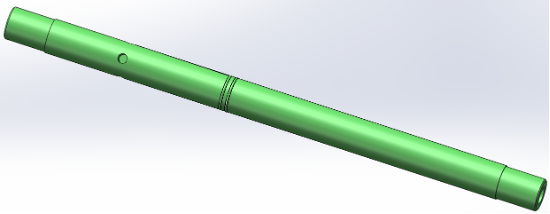
\includegraphics[width=0.7\textwidth]{figure/chapter3/inner-pipe-3-in-1.png}
	}
	\hfill
	\subfloat[抗拉强度分析]{%
	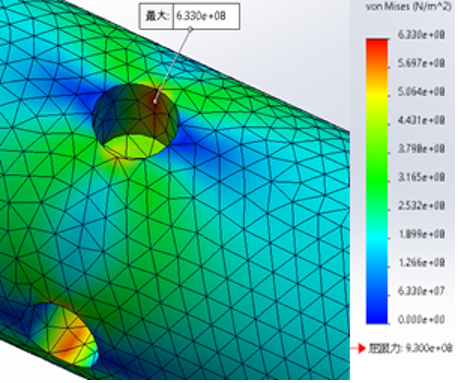
\includegraphics[width=0.4\textwidth]{figure/chapter3/inner-pipe-3-in-1-tensile-stress.png}
	}
	\vspace{1em}
	\subfloat[抗扭强度分析]{%
	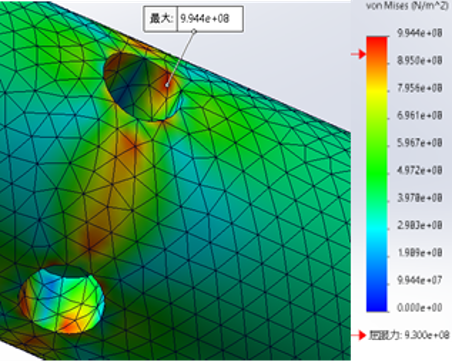
\includegraphics[width=0.45\textwidth]{figure/chapter3/inner-pipe-3-in-1-torsional-stress.png}
	}
	\caption{脉冲发生器薄弱零件强度有限元分析}
	\label{fig:FEA_inner_pipe_3_in_1}
\end{figure}